\mySection{14.6 Testing for Randomness}
%Introduction-------------- start slide -------------------------------%{{{ 14.6
\begin{frame}
	\begin{itemize}
		\item[] Whether the sample are random at all?
		\item[E.g.] Whether the number of successful strikes are random? $\alpha=0.05$.
		\begin{center}
			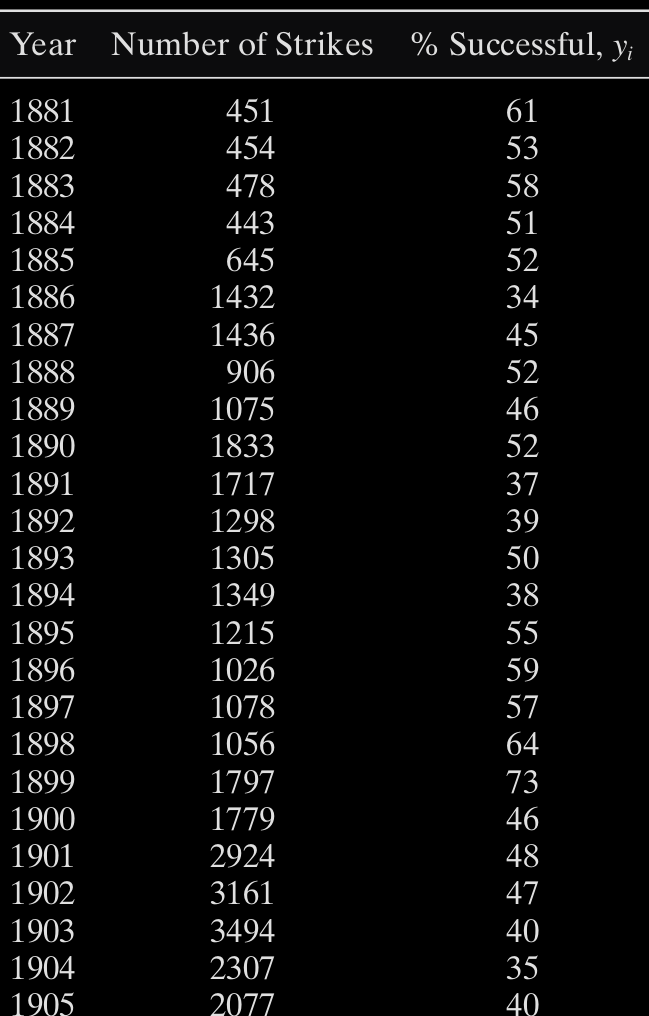
\includegraphics[scale=0.2]{Codes/Table14-6-1_1.png}
		\end{center}
	\end{itemize}
\end{frame}
%-------------- end slide -------------------------------%}}}
%-------------- start slide -------------------------------%{{{ 1
\begin{frame}[fragile]
\begin{itemize}
	\item[Sol.] Compute the run-up and run-down:
		\begin{center}
		\def\x{0.275}
	\begin{tikzpicture}[scale=1, transform shape]
			\node (fig) at (0,0) {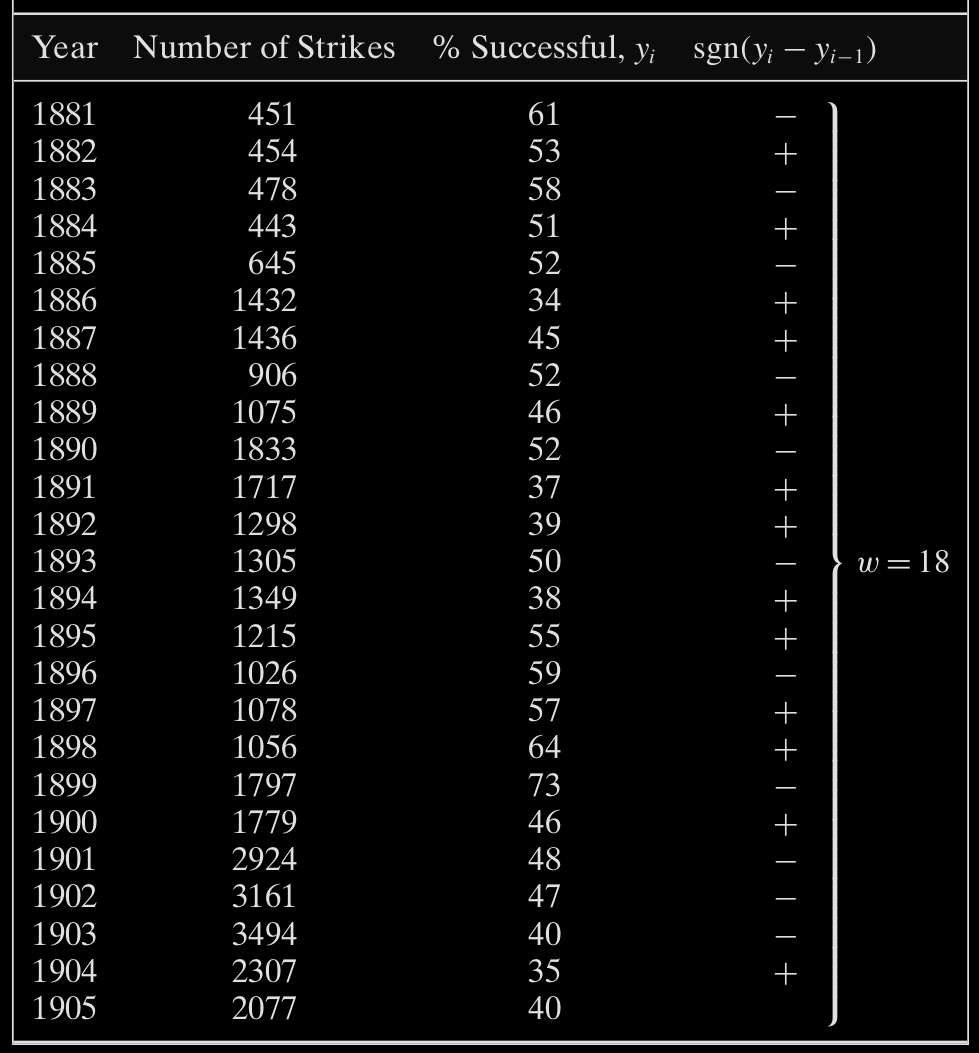
\includegraphics[scale=0.2]{Codes/Table14-6-1.png}};
			\draw[red,->] (1.5,2.9) node [left] {$1$} -- ++(0.3,0) ;
			\draw[red,->] (1.5,2.65) node [left] {$2$} -- ++(0.3,0) ;
			\draw[red,->] (1.5,2.65-\x) node [left] {$3$} -- ++(0.3,0) ;
			\draw[red,->] (1.5,2.65-2*\x) node [left] {$4$} -- ++(0.3,0) ;
			\draw[red,->] (1.5,2.65-3*\x) node [left] {$5$} -- ++(0.3,0) ;
			\draw[red,->] (1.5,2.65-4*\x) node [left] {$6$} -- ++(0.3,0) ;
			\draw[red,->] (1.5,2.65-6*\x) node [left] {$7$} -- ++(0.3,0) ;
			\draw[red,->] (1.5,0.78) node [left] {$8$} -- ++(0.3,0) ;
			\draw[red,->] (1.5,0.78-\x) node [left] {$9$} -- ++(0.3,0) ;
			\draw[red,->] (1.5,0.78-2*\x) node [left] {$10$} -- ++(0.3,0) ;
			\draw[red,->] (1.5,-0.26) node [left] {$11$} -- ++(0.3,0) ;
			\draw[red,->] (1.5,-0.26-\x) node [left] {$12$} -- ++(0.3,0) ;
			\draw[red,->] (1.5,-1.07) node [left] {$13$} -- ++(0.3,0) ;
			\draw[red,->] (1.5,-1.07-\x) node [left] {$14$} -- ++(0.3,0) ;
			\draw[red,->] (1.5,-1.85) node [left] {$15$} -- ++(0.3,0) ;
			\draw[red,->] (1.5,-1.85-\x) node [left] {$16$} -- ++(0.3,0) ;
			\draw[red,->] (1.5,-1.85-2*\x) node [left] {$17$} -- ++(0.3,0) ;
			\draw[red,->] (1.5,-3.15) node [left] {$18$} -- ++(0.3,0) ;
		\end{tikzpicture}
		\end{center}
\end{itemize}
\end{frame}
%-------------- end slide -------------------------------%}}}
%-------------- start slide -------------------------------%{{{ 1
\begin{frame}[fragile]
\begin{itemize}
	\item[Theorem] Let $W$ be the number of runs up and down in a sequence of $n\ge 2$ observations.
	\item[] If the sequence is random, then
	\begin{align*}
		\E(W)=\frac{2n-1}{3} \quad\text{and}\quad \Var(W)= \frac{16n-29}{90}.
	\end{align*}
	\item[] Moreover, when $n$ is large, namely,  $n\ge 20$, then
	\bigskip
	 \begin{align*}
		\frac{W-\E(W)}{\sqrt{\Var(W)}} = \frac{W-[2n-1]/3}{\sqrt{[16n-29]/90}}\quad\stackrel{approx}{\sim}\quad N(0,1).
	\end{align*}
	\end{itemize}
\end{frame}
%-------------- end slide -------------------------------%}}}
%-------------- start slide -------------------------------%{{{ 1
\begin{frame}[fragile]
\begin{itemize}
	\item[Sol.] (Continued) $n=25$,  $w=18$
	\begin{align*}
		\E(W) = \frac{2\times 25 -1}{3} = 16.3
	\end{align*}
	and
	\begin{align*}
		\Var(W) = \frac{16 \times 25 -29}{90} =4.12.
	\end{align*}
	\item[] Hence, the z-score is
	\begin{align*}
		z=\frac{18-16.3}{\sqrt{4.12}} = 0.84.
	\end{align*}
	\item[] The critical region is
	\begin{align*}
		C = \left\{z: |z|\ge z_{\alpha/2} =z_{0.025}= 1.96\right\}
	\end{align*}
	\item[] The $p$-value is
		 \begin{align*}
			 2 \times\bbP(Z > 0.84) = 0.4009084
			 % R Code
		   %
			 % 2*(1-pnorm(0.84))
       %
		\end{align*}
	\item[] Conclusion: Fail to reject. \myQED
\end{itemize}
\end{frame}
%-------------- end slide -------------------------------%}}}
%-------------- start slide -------------------------------%{{{ 1
\begin{frame}[fragile]
	\begin{minipage}{0.45\textwidth}
			R code:
		\begin{lstlisting}
library("snpar")
y <- c(0,1,0,1,0,1,1,0,1,0,1,1,
	0,1,1,0,1,1,0,1,0,0,0,1)
runs.test(y, exact = FALSE)
runs.test(y, exact = TRUE)
		\end{lstlisting}
	\end{minipage}
	\hfill
	\begin{minipage}{0.45\textwidth}
Output:
\begin{lstlisting}
> runs.test(y, exact = FALSE)

        Approximate runs rest

data:  y
Runs = 18, p-value = 0.03256
alternative hypothesis: two.sided

> runs.test(y, exact = TRUE)

        Exact runs test

data:  y
Runs = 18, p-value = 0.01624
alternative hypothesis: two.sided
\end{lstlisting}
	\end{minipage}
\vfill
%
%
% library("snpar")
% x <- c(
% 61, 53, 58, 51, 52, 34, 45, 52, 46, 52, 37, 39, 50,
% 38, 55, 59, 57, 64, 73, 46, 48, 47, 40, 35, 40)
% runs.test(x, exact = TRUE )
% runs.test(x, exact = FALSE )
%
% library("randtests")
% x <- c(13, 3, 14, 14, 1, 14, 3, 8, 14, 17, 9, 14, 13, 2, 16, 1, 3, 12, 13, 14)
% RunsTest(x)
%
% install.packages("randtests")
%
%
% (18-(2*25-1)/3)/sqrt((16*25-29)/90)
\begin{itemize}
		\item[Remark] The procedure that we learnt is an approximation. There is a big discrepancy for the above two $p$-values:
			one that we obtained through formula and one that is obtained by the r function.
	\end{itemize}
\end{frame}
%-------------- end slide -------------------------------%}}}
%-------------- start slide -------------------------------%{{{ 1
\begin{frame}[fragile]
\begin{center}
\begin{minipage}{0.6\textwidth}
\centering
\huge
Thanks for learning statistics with me through the semester~!
\end{minipage}
\end{center}
\end{frame}
%-------------- end slide -------------------------------%}}}
